\documentclass[11pt]{article}
\usepackage{theme}
\usepackage{shortcuts}
% Document parameters
% Document title
\title{Assignment 1 (ML for TS) - MVA 2023/2024}
\author{
Yvann Le Fay \email{yvann.lefay@ensae.fr} \\ % student 1
Antoine Schoonaert \email{antoine.schoonaert@etu.emse.fr} % student 2
}

\begin{document}
\maketitle

\section{Introduction}

\paragraph{Objective.} This assignment has three parts: questions about the convolutional dictionary learning, the spectral features and a data study using the DTW.

\paragraph{Warning and advice.}
\begin{itemize}
    \item Use code from the tutorials as well as from other sources. Do not code yourself well-known procedures (e.g. cross validation or k-means), use an existing implementation.
    \item The associated notebook contains some hints and several helper functions.
    \item Be concise. Answers are not expected to be longer than a few sentences (omitting calculations).
\end{itemize}



\paragraph{Instructions.}
\begin{itemize}
    \item Fill in your names and emails at the top of the document.
    \item Hand in your report (one per pair of students) by Tuesday 7\textsuperscript{th} November 23:59 PM.
    \item Rename your report and notebook as follows:\\ \texttt{FirstnameLastname1\_FirstnameLastname2.pdf} and\\ \texttt{FirstnameLastname1\_FirstnameLastname2.ipynb}.\\
    For instance, \texttt{LaurentOudre\_CharlesTruong.pdf}.
    \item Upload your report (PDF file) and notebook (IPYNB file) using this link: \footnotesize{\href{https://docs.google.com/forms/d/e/1FAIpQLSdTwJEyc6QIoYTknjk12kJMtcKllFvPlWLk5LbyugW0YO7K6Q/viewform?usp=sf_link}{docs.google.com/forms/d/e/1FAIpQLSdTwJEyc6QIoYTknjk12kJMtcKllFvPlWLk5LbyugW0YO7K6Q/viewform?usp=sf\_link}}.
\end{itemize}


\section{Convolution dictionary learning}

\begin{exercise}
Consider the following Lasso regression:
\begin{equation}\label{eq:lasso}
    \min_{\beta\in\RR^p} \frac{1}{2}\norm{y-X\beta}^2_2 \quad + \quad \lambda \norm{\beta}_1
\end{equation}
where $y\in\RR^n$ is the response vector, $X\in\RR^{n\times p}$ the design matrix, $\beta\in\RR^p$ the vector of regressors and $\lambda>0$ the smoothing parameter.

Show that there exists $\lambda_{\max}$ such that the minimizer of~\eqref{eq:lasso} is $\mathbf{0}_p$ (a $p$-dimensional vector of zeros) for any $\lambda > \lambda_{\max}$.
\end{exercise}

\begin{solution}
Let $\mathcal{L} : \beta\in\mathbb{R}^p\mapsto \frac{1}{2}\norm{y-X\beta}^2_2+\lambda \norm{\beta}_1$, this is a non-differentiable (because of the $l_1$-norm term) convex function. Its subdifferential is given by
%
\begin{equation}
    \partial \mathcal{L}(\beta) = -X^{\top}(y-X\beta)+\lambda\partial\norm{\beta}_1,
\end{equation}
%
where the subdifferential of the $l_1$-norm is given by
%
\begin{equation}
    \partial\norm{\beta}_1 = \{z\in \mathbb{R}^p : z_j = \text{sgn}(\beta) \text{ if } \beta_j\neq 0, z_j\in [-1, 1] \text{ if } x_j = 0\}.
\end{equation}
%
The first-order optimality implies at the optimal $\beta(\lambda)$, there exists $z^{*}\in \partial \norm{\beta(\lambda)}_1$ such that
%
\begin{equation}
    X^{\top}(y-X\beta(\lambda)) + \lambda z^{*} = 0,
\end{equation}
%
i.e.,
%
\begin{equation}
    X^{\top}X \beta(\lambda ) = X^{\top}y-\lambda z^{*}.
\end{equation}
%
Thus, we have
%
\begin{equation}
\begin{split}
    0 \leq \beta(\lambda)X^{\top}X\beta(\lambda) &= \langle \beta(\lambda), X^{\top}y-\lambda z^{*}\rangle\\
    &=\sum_{j/ \beta(\lambda)_j\neq 0}\beta(\lambda)_j (X^{\top}_j y - \lambda \text{sgn}(\beta(\lambda)_j),
\end{split}
\end{equation}
%
where the $X_j$'s are the columns of $X$ and the $\beta(\lambda)_j$'s are are the components of $\beta(\lambda)$.
The previous inequality implies that for $\lambda \geq \max_{j\in [1, p]} |X^{\top}_jy|$, $\beta(\lambda)_j = 0$ (however, it does not seem trivial to show that it is a the minimal $\lambda$ such that $\beta(\lambda)$ is 0). Thus, for any $\lambda\geq \lambda_{max}$, where
\begin{equation}
    \lambda_{\max} =  \max_{j\in [1, p]} |X^{\top}_jy|,
\end{equation}
we have $\beta(\lambda)= 0$.

\end{solution}

\begin{exercise}
For a univariate signal $\mathbf{x}\in\mathbb{R}^n$ with $n$ samples, the convolutional dictionary learning task amounts to solving the following optimization problem:

\begin{equation}
\min_{(\mathbf{d}_k)_k, (\mathbf{z}_k)_k \\ \norm{\mathbf{d}_k}_2^2\leq 1} \quad\norm{\mathbf{x} - \sum_{k=1}^K \mathbf{z}_k * \mathbf{d}_k }^2_2 \quad + \quad\lambda \sum_{k=1}^K \norm{\mathbf{z}_k}_1
\end{equation}

where $\mathbf{d}_k\in\mathbb{R}^L$ are the $K$ dictionary atoms (patterns), $\mathbf{z}_k\in\mathbb{R}^{N-L+1}$ are activations signals, and $\lambda>0$ is the smoothing parameter.

Show that
\begin{itemize}
    \item for a fixed dictionary, the sparse coding problem is a lasso regression (explicit the response vector and the design matrix);
    \item for a fixed dictionary, there exists $\lambda_{\max}$ (which depends on the dictionary) such that the sparse codes are only 0 for any $\lambda > \lambda_{\max}$.
\end{itemize}
\end{exercise}

\begin{solution}
We have $\sum_{k=1}^{K} (\mathbf{z}_k * \mathbf{d}_k)(i) = \sum_{k=1}^{K}\sum_{j=0}^{L-1}\mathbf{z}_k(j) \mathbf{d}_k(i-j)$ which can we rewritten $\sum_{k=1}^{K} \mathbf{z}_k* \mathbf{d}_k = Dz$ where
%
\begin{equation}
    D = (D_1, \ldots, D_K),\quad z=[\mathbf{z}_1^{\top}, \ldots, \mathbf{z}_K^{\top}]^{\top},
\end{equation}
%
and where the $D_i$'s are Toeplitz matrices for the convolution product by the $\mathbf{d}_i$'s, i.e.,
%
\begin{equation}
    D_i = \begin{pmatrix}
        d_i(0) & 0 & \ldots& 0 & 0\\
        d_i(1) & d_i(0) & &\hdots & \hdots\\
        d_i(2) & d_i(1) & \ldots & 0 & 0\\
        \hdots & d_i(2) & \ldots & d_i(0) & 0\\
        d_i(L-2) & \hdots &\ddots & d_i(1) & d_i(0)\\
        d_i(L-1) & d_i(L-2) & & \vdots & d_i(1)\\
        0 & d_i(L-1) &\ddots & d_i(L-3) & \vdots\\
        0 & 0 & \ldots & d_i(L-2) & d_i(L-3)\\
        \vdots & \vdots & & d_i(L-1) & d_i(L-2)\\
        0 & 0& 0 &\ldots & d_i(L-1)

    \end{pmatrix}.
\end{equation}
%
In that case, using the result of the previous question, we have
%
\begin{equation}
    \lambda_{max} = \max_{i\in[1, K]}{\norm{D_i^{\top}\mathbf{x}}_{\infty}}.
\end{equation}
%
\end{solution}

\section{Spectral feature}

Let $X_n$ ($n=0,\dots,N-1)$ be a weakly stationary random process with zero mean and autocovariance function $\gamma(\tau):= \mathbb{E}(X_n X_{n+\tau})$.
Assume the autocovariances are absolutely summable, \ie $\sum_{\tau\in\mathbb{Z}} |\gamma(\tau)| < \infty$, and square summable, \ie $\sum_{\tau\in\mathbb{Z}} \gamma^2(\tau) < \infty$.
Denote by $f_s$ the sampling frequency, meaning that the index $n$ corresponds to the time instant $n / f_s$ and for simplicity, let $N$ be even.


The \textit{power spectrum} $S$ of the stationary random process $X$ is defined as the Fourier transform of the autocovariance function:
\begin{equation}
    S(f) := \sum_{\tau=-\infty}^{+\infty}\gamma(\tau)e^{-2i\pi f\tau/f_s}.
\end{equation}
The power spectrum describes the distribution of power in the frequency space.
Intuitively, large values of $S(f)$ indicates that the signal contains a sine wave at the frequency $f$.
There are many estimation procedures to determine this important quantity, which can then be used in a machine learning pipeline.
In the following, we discuss about the large sample properties of simple estimation procedures, and the relationship between the power spectrum and the autocorrelation.

(Hint: use the many results on quadratic forms of Gaussian random variables to limit the amount of calculations.)

\begin{exercise}
In this question, let $X_n$ ($n=0,\dots,N-1)$ be a Gaussian white noise.

\begin{itemize}
    \item Calculate the associated autocovariance function and power spectrum. (By analogy with the light, this process is called ``white'' because of the particular form of its power spectrum.)
\end{itemize}

\end{exercise}

\begin{solution}
    Let $X_n \overset{\mathrm{iid}}{\sim} \mathcal{N}(0, \sigma^2)$ ($n=0,\ldots, N-1)$, then the autocovariance function is given, for any $\tau\in [0, N-1]$, by
    \begin{equation}
        \gamma(\tau) = \mathbb{E}(X_0 X_{\tau}) =  \left\{
    \begin{array}{ll}
        \sigma^2 & \tau = 0 \\
        0 & \tau \neq 0
    \end{array},
\right.
    \end{equation}
    and the power spectrum is given by
    \begin{equation}
        S = \sigma^2.
    \end{equation}
\end{solution}


\begin{exercise}
A natural estimator for the autocorrelation function is the sample autocovariance
\begin{equation}
    \hat{\gamma}(\tau) := (1/N) \sum_{n=0}^{N-\tau-1} X_n X_{n+\tau}
\end{equation}
for $\tau=0,1,\dots,N-1$ and $\hat{\gamma}(\tau):=\hat{\gamma}(-\tau)$ for $\tau=-(N-1),\dots,-1$.
\begin{itemize}
    \item Show that $\hat{\gamma}(\tau)$ is a biased estimator of $\gamma(\tau)$ but asymptotically unbiased.
    What would be a simple way to de-bias this estimator?
\end{itemize}

\end{exercise}

\begin{solution}
Let $\tau \in [0, N-1]$, we have
\begin{equation}
    \begin{split}
        \mathbb{E}[\hat{\gamma}(\tau)] &= \frac{1}{N}\sum_{n=0}^{N-\tau-1}\mathbb{E}[X_n X_{n+\tau}]\\
                                    &= \frac{N-\tau}{N}\gamma(\tau),
    \end{split}
\end{equation}
which is biased up to a multiplicative constant, except for $\tau = 0$. As $N$ goes to infinity, the multiplicative constant $\frac{N-\tau}{N}$ goes to $1$, which shows that the estimator is asymptotically unbiased. Let $\hat{\gamma}^* = \frac{N}{N-\tau}\hat{\gamma}$, this is an de-biased version of the previous estimator.
\end{solution}

\begin{exercise}
Define the discrete Fourier transform of the random process $\{X_n\}_n$ by
\begin{equation}
    J(f) := (1/\sqrt{N})\sum_{n=0}^{N-1} X_n e^{-2\pi\iu f n/f_s}
\end{equation}
The \textit{periodogram} is the collection of values $|J(f_0)|^2$, $|J(f_1)|^2$, \dots, $|J(f_{N/2})|^2$ where $f_k = f_s k/N$.
(They can be efficiently computed using the Fast Fourier Transform.)
\begin{itemize}
    \item Write $|J(f_k)|^2$ as a function of the sample autocovariances.
    \item For a frequency $f$, define $f^{(N)}$ the closest Fourier frequency $f_k$ to $f$.
    Show that $|J(f^{(N)})|^2$ is an asymptotically unbiased estimator of $S(f)$ for $f>0$.
\end{itemize}
\end{exercise}

\begin{solution}
Let $k \in \mathbb{N}$, we have
    %
    \begin{equation}
        \begin{split}
            |J(f_k)|^2 &= J(f_k)\overline{J(f_k)}\\
            &= \frac{1}{N}\sum_{n, m = 0}^{N-1} X_n X_m e^{-2\pi i k(n-m)/N}\\
            & = \frac{1}{N}\sum_{n=0,m=0}^{N-1}\sum_{\tau=-(N-1)}^{N-1} \mathds{1}(n-m=\tau) X_n X_m e^{-2\pi i k(n-m)/N}\\
            &= \frac{1}{N}\bigg\{\sum_{\tau=1}^{N-1}\sum_{m=0}^{N-1-\tau}X_{m+\tau}X_m e^{-2i\pi k /N \tau}+\sum_{\tau=1}^{N-1}\sum_{n=0}^{N-1-\tau}X_n X_{n+\tau}e^{2i\pi k/N \tau} + \sum_{n=0}^{N-1} X_n^2\bigg\}\\
            &= \frac{1}{N}\bigg\{2\sum_{\tau=1}^{N-1}\cos{\big(2\pi k / N \tau\big)}\sum_{n=0}^{N-1-\tau}X_nX_{n+\tau}+\sum_{n=0}^{N-1}X_n^2\bigg\}\\
            &= 2\sum_{\tau=1}^{N-1}\cos{\big(2\pi k / N \tau\big)}\hat{\gamma}(\tau) + \hat{\gamma}(0)\\
            &= \sum_{\tau=-(N-1)}^{N-1}e^{-2i\pi k / N \tau}\hat{\gamma}(\tau),
        \end{split}
    \end{equation}
    %
    where we used $\gamma(\tau) = \gamma(-\tau)$ for $\tau \in [-(N-1), -1]$ for the last line.
    Using the previous result and formally computing the expectation, we have for $k(f)$ realising the $f_{k(f)} = f^{(N)}$
    %
    \begin{equation}
        \begin{split}
            \mathbb{E}[|J(f^{(N)})|^2] = \sum_{\tau=-(N-1)}^{N-1}e^{-2i\pi k(f) /N \tau}(1-\tau/N)\gamma(\tau).
        \end{split}
    \end{equation}
    %
    Since the autocovariances are absolutely summable, and $k(f)/N$ converges to $f/f_s$, the sum converges uniformly to $S(f)$.
    %
\end{solution}

\begin{exercise}\label{ex:wn-exp}
    In this question, let $X_n$ ($n=0,\dots,N-1)$ be a Gaussian white noise with variance $\sigma^2=1$ and set the sampling frequency to $f_s=1$ Hz
    \begin{itemize}
        \item For $N\in\{200, 500, 1000\}$, compute the \textit{sample autocovariances} ($\hat{\gamma}(\tau)$ vs $\tau$) for 100 simulations of $X$.
        Plot the average value as well as the average $\pm$ the standard deviation.
        What do you observe?
        \item For $N\in\{200, 500, 1000\}$, compute the \textit{periodogram} ($|J(f_k)|^2$ vs $f_k$) for 100 simulations of $X$.
        Plot the average value as well as the average $\pm$ the standard deviation.
        What do you observe?
    \end{itemize}
    Add your plots to Figure~\ref{fig:wn-exp}.

\begin{figure}
    \centering
    \begin{minipage}[t]{0.3\textwidth}
    \centerline{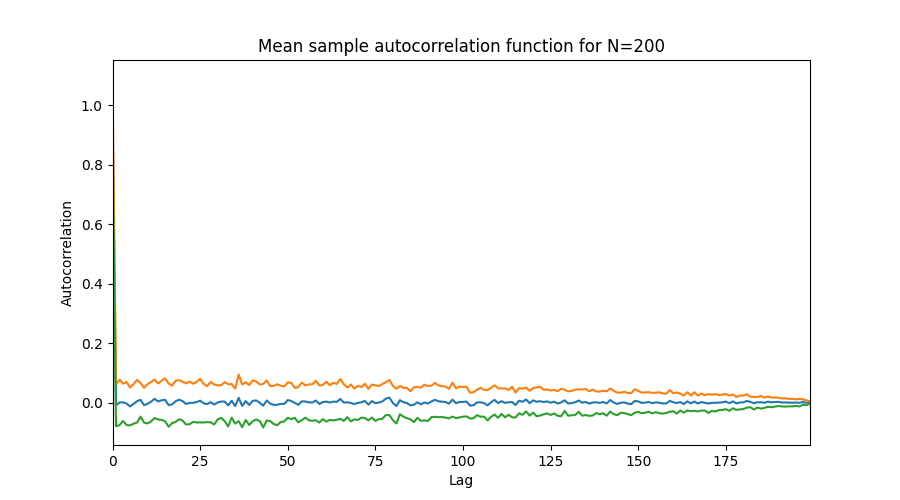
\includegraphics[width=\textwidth]{Assignment 1 - ML for TS (MVA 2023-2024)/mean_sample_autocorrelation_N=200.png}}
    \centerline{Autocovariance ($N=200$)}
    \end{minipage}
    \begin{minipage}[t]{0.3\textwidth}
    \centerline{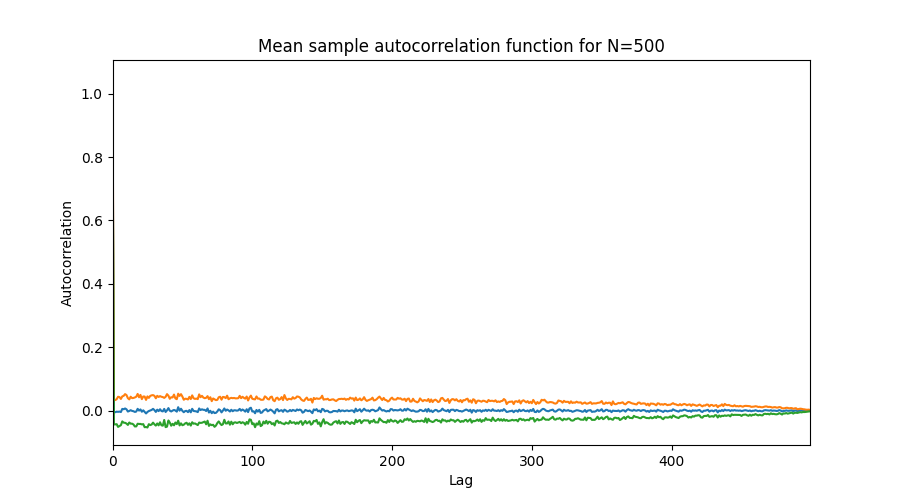
\includegraphics[width=\textwidth]{Assignment 1 - ML for TS (MVA 2023-2024)/mean_sample_autocorrelation_N=500.png}}
    \centerline{Autocovariance ($N=500$)}
    \end{minipage}
    \begin{minipage}[t]{0.3\textwidth}
    \centerline{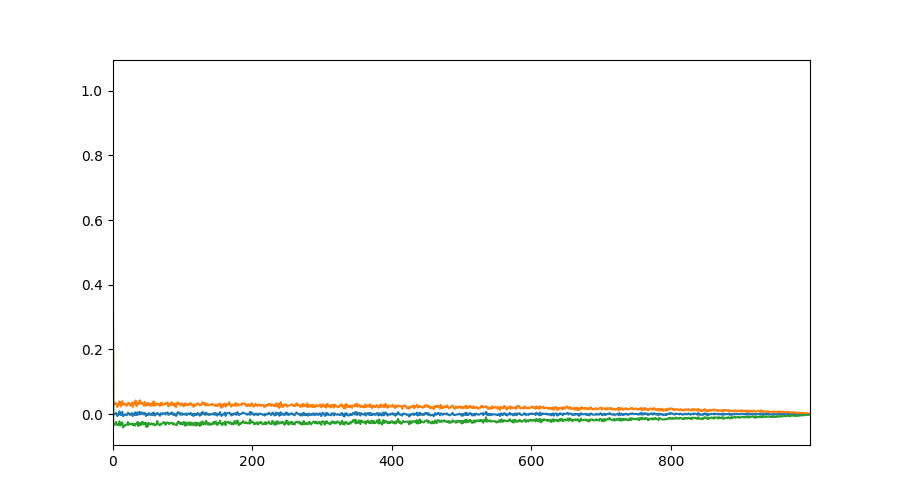
\includegraphics[width=\textwidth]{Assignment 1 - ML for TS (MVA 2023-2024)/mean_sample_autocorrelation_N=1000.png}}
    \centerline{Autocovariance ($N=1000$)}
    \end{minipage}
    \vskip1em
    \begin{minipage}[t]{0.3\textwidth}
    \centerline{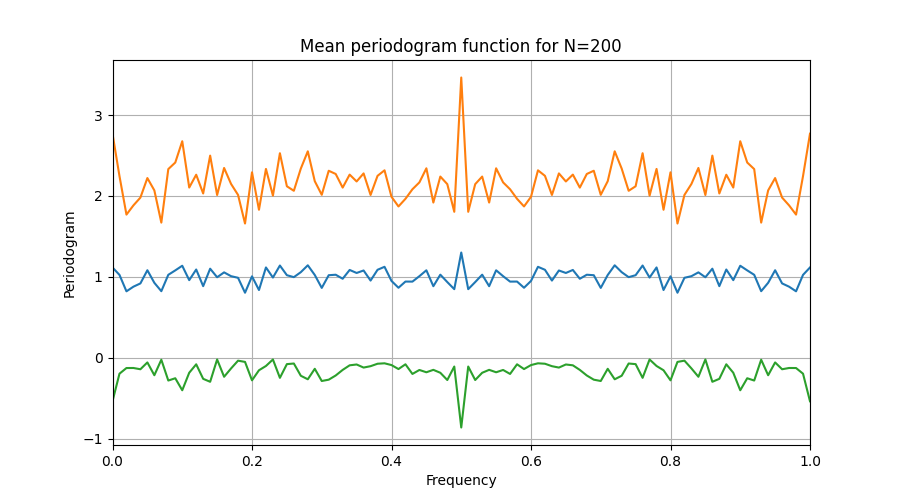
\includegraphics[width=\textwidth]{Assignment 1 - ML for TS (MVA 2023-2024)/mean_periodogram_N=200.png}}
    \centerline{Periodogram ($N=200$)}
    \end{minipage}
    \begin{minipage}[t]{0.3\textwidth}
    \centerline{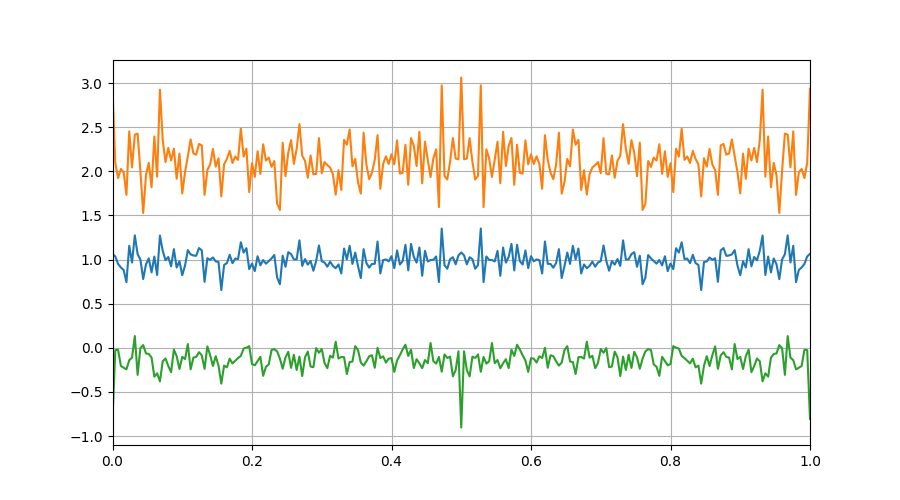
\includegraphics[width=\textwidth]{Assignment 1 - ML for TS (MVA 2023-2024)/mean_periodogram_N=500.png}}
    \centerline{Periodogram ($N=500$)}
    \end{minipage}
    \begin{minipage}[t]{0.3\textwidth}
    \centerline{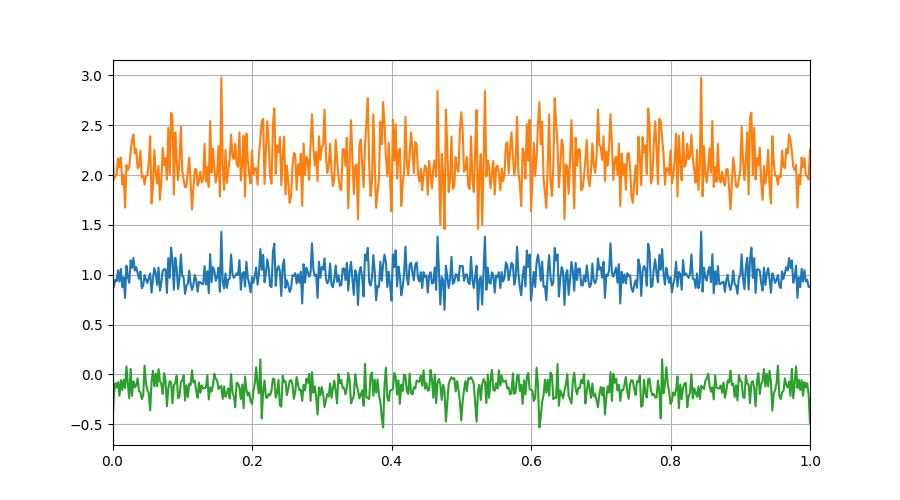
\includegraphics[width=\textwidth]{Assignment 1 - ML for TS (MVA 2023-2024)/mean_periodogram_N=1000.png}}
    \centerline{Periodogram ($N=1000$)}
    \end{minipage}
    \vskip1em
    \caption{Autocovariances and periodograms of a Gaussian white noise (see Question~\ref{ex:wn-exp}).}
    \label{fig:wn-exp}
\end{figure}

\end{exercise}

\begin{solution}

\end{solution}

\begin{exercise}
    We want to show that the estimator $\hat{\gamma}(\tau)$ is consistent, \ie it converges in probability when the number $N$ of samples grows to $\infty$ to the true value ${\gamma}(\tau)$.
    In this question, assume that $X$ is a wide-sense stationary \textit{Gaussian} process.
    \begin{itemize}
        \item Show that for $\tau>0$
    \begin{equation}
       \text{var}(\hat{\gamma}(\tau)) = (1/N) \sum_{n=-(N-\tau-1)}^{n=N-\tau-1} \left(1 - \frac{\tau + |n|}{N}\right) \left[\gamma^2(n) + \gamma(n-\tau)\gamma(n+\tau)\right].
    \end{equation}
    (Hint: if $\{Y_1, Y_2, Y_3, Y_4\}$ are four centered jointly Gaussian variables, then $\mathbb{E}[Y_1 Y_2 Y_3 Y_4] = \mathbb{E}[Y_1 Y_2]\mathbb{E}[Y_3 Y_4] + \mathbb{E}[Y_1 Y_3]\mathbb{E}[Y_2 Y_4] + \mathbb{E}[Y_1 Y_4]\mathbb{E}[Y_2 Y_3]$.)
    \item Conclude that $\hat{\gamma}(\tau)$ is consistent.
    \end{itemize}
\end{exercise}

\begin{solution}
    Let us compute the variance, using the above equality to go from the first to the second line, we have for $\tau > 0$
    %
    \begin{equation}
        \begin{split}
            \mathbb{E}[\hat{\gamma}^2(\tau)] &= \frac{1}{N^2}\sum_{n,m=0}^{N-\tau-1}\mathbb{E}[X_{n}X_{n+\tau}X_mX_{m+\tau}]\\
            &= \frac{1}{N^2}\sum_{n,m=0}^{N-\tau-1}\{\mathbb{E}[X_nX_{n+\tau}]\mathbb{E}[X_mX_{m+\tau}]+\mathbb{E}[X_nX_{m}]\mathbb{E}[X_{n+\tau}X_{m+\tau}]+\mathbb{E}[X_nX_{m+\tau}]\mathbb{E}[X_mX_{n+\tau}]\}\\
            &= \frac{1}{N^2}\sum_{n,m=0}^{N-\tau-1}\{\gamma(\tau)^2 + \gamma(m-n)^2 + \gamma(n+\tau-m)\gamma(m+\tau-n)\}.
        \end{split}
    \end{equation}
    %
    Thus, substracting $\mathbb{E}[\hat{\gamma}(\tau)]^2 = (1-\tau/N)^2\gamma(\tau)^2 = \frac{1}{N^2}\sum_{n,m=0}^{N-\tau+1} \gamma(\tau)^2$, we have
    %
    \begin{equation}
    \begin{split}
        \text{var}(\hat{\gamma}(\tau)) &= \frac{1}{N^2}\sum_{n,m=0}^{N-\tau-1}\gamma(m-n)^2 + \gamma(n+\tau-m)\gamma(m+\tau-n)\\
        &= \frac{1}{N^2}\sum_{n=0}^{N-\tau-1}\sum_{m=0}^{N-\tau-1}\big\{\sum_{k=-(N-\tau-1)}^{N-\tau-1}\mathds{1}(m-n=k)\big\} (\gamma^2(k)+\gamma(k-\tau)\gamma(\tau+k))\\
        &=\frac{1}{N^2}\sum_{k=-(N-\tau-1)}^{N-\tau-1} \text{card}((m,n)\in [0, N-\tau-1]^2 / m-n=k) (\gamma^2(k)+\gamma(k-\tau)\gamma(\tau+k))\\
        &= \frac{1}{N^2}\sum_{k=-(N-\tau-1)}^{N-\tau-1} (N-\tau-|k|)(\gamma^2(k)+\gamma(k-\tau)\gamma(\tau+k))\\
        &= \frac{1}{N}\sum_{k=-(N-\tau-1)}^{N-\tau-1} (1-\frac{\tau+|k|}{N})(\gamma^2(k)+\gamma(k-\tau)\gamma(\tau+k))\\
        &\leq \frac{1}{N}\sum_{k=-(N-\tau-1)}^{N-\tau-1}\gamma^2(k)+|\gamma(k-\tau)\gamma(\tau+k)|\\
        &\leq \frac{1}{N}\bigg(\sum_{k=-(N-\tau-1)}^{N-\tau-1}\gamma^2(k) + \sqrt{\sum_{k=-(N-\tau-1)}^{N-\tau-1}\gamma^2(k-\tau)\sum_{k=-(N-\tau-1)}^{N-\tau-1}\gamma^2(\tau+k)}\bigg)\\
        &\leq \frac{2}{N}\sum_{k\in\mathbb{Z}}\gamma^2(k),
    \end{split}
    \end{equation}
    %
    where to go from the first to the second line, we used $\gamma(k-\tau)=\gamma(\tau-k)$, computing the cardinal of pairs $(m,n)\in [0, N-\tau-1]^2$ such that $m-n = k$ can be done by a quick drawing, one obtains $N-\tau-|k|$. This is the desired result.

    Now, let us prove that the estimator is indeed consistent by using Bienaymé-Tcheybychev inequality. For any $t>0$, we have
    %
    \begin{equation}
        \begin{split}
            \mathbb{P}[|\hat{\gamma}(\tau)-\gamma(\tau)|>t]&\leq \frac{\text{var}(\hat{\gamma}(\tau))}{t^2}\\
            &\leq \frac{c}{Nt^2},
        \end{split}
    \end{equation}
    %
    where $c=2\sum_{n\in\mathbb{Z}}\gamma^2(n)$ is finite because the autocovariances are square-summable. Hence, for any $t > 0$, $\mathbb{P}[\hat{\gamma}(\tau)-\gamma(\tau)|>t]$ goes to $0$ as $N$ goes to $\infty$, which exactly means that $\hat{\gamma}(\tau)$ is consistent.
    %
\end{solution}

Contrary to the correlogram, the periodogram is not consistent.
It is one of the most well-known estimators that is asymptotically unbiased but not consistent.
In the following question, this is proven for a Gaussian white noise but this holds for more general stationary processes.
\begin{exercise}
    Assume that $X$ is a Gaussian white noise (variance $\sigma^2$) and let $A(f):=\sum_{n=0}^{N-1} X_n \cos(-2\pi f n/f_s)$ and $B(f):=\sum_{n=0}^{N-1} X_n \sin(-2\pi f n/f_s)$.
    Observe that $J(f) = (1/\sqrt{N}) (A(f) + \iu B(f))$.
    \begin{itemize}
        \item Derive the mean and variance of $A(f)$ and $B(f)$ for $f=f_0, f_1,\dots, f_{N/2}$ where $f_k=f_s k/N$.
        \item What is the distribution of the periodogram values $|J(f_0)|^2$, $|J(f_1)|^2$, \dots, $|J(f_{N/2})|^2$.
        \item What is the variance of the $|J(f_k)|^2$? Conclude that the periodogram is not consistent.
        \item Explain the erratic behavior of the periodogram in Question~\ref{ex:wn-exp} by looking at the covariance between the $|J(f_k)|^2$.
    \end{itemize}

\end{exercise}

\begin{solution}
    Since the $X_n$'s have zero-mean, we obtain that $\mathbb{E}[A(f)] = \mathbb{E}[B(f)] = 0$. Let us compute the variance of $A(f_k)$ for $k\in [0, N/2]$, using the mutual independence of the $X_n$'s and trigonometric formulas,
    %
    \begin{equation}
        \begin{split}
            \text{var}(A(f_k)) &= \sum_{n=0}^{N-1}\text{var}(X_n \cos(-2\pi k n / N))\\
            &=\sigma^2\sum_{n=0}^{N-1}\cos^2(-2\pi k n/N )\\
            &=\frac{\sigma^2}{2}\sum_{n=0}^{N-1}(\cos(-4\pi k n / N)+1)\\
            &=\frac{\sigma^2N}{2}.
        \end{split}
    \end{equation}
    %
    Similarly, we have
    %
    \begin{equation}
        \begin{split}
            \text{var}(B(f_k)) &= \frac{\sigma^2N}{2}.
        \end{split}
    \end{equation}
    %
    Moreover, we have
    %
    \begin{equation}
        \begin{split}
            \mathbb{E}[A(f_k)B(f_k)] &= \mathbb{E}[\sum_{n,m=0}^{N-1}X_nX_m\cos(-2\pi k n / N)\sin(-2\pi k m / N)]\\ &= \sigma^2\sum_{n=0}^{N-1}\cos(-2\pi k n / N)\sin(-2\pi k n / N)\\
            &= -\frac{\sigma^2}{2}\sum_{n=0}^{N-1}\sin(4\pi k n / N)\\
            &= -\frac{\sigma^2}{2}\text{Im}\sum_{n=0}^{N-1}e^{4\pi i k n /N}\\
            &= -\frac{\sigma^2}{2}(\text{Im}(1 + e^{2\pi i k}))+\sum_{n=1}^{N/2-1}\text{Im}(e^{4\pi i k n / N}+e^{4\pi i k (N-n)/N}))\\
            &= 0,
        \end{split}
    \end{equation}
    %
    where we remark that $e^{4\pi i k n / N}$ is the conjugate of $e^{4\pi i k (N-n)/N}$ and similar arguments were used for the two previous variances.
    Since, $A$ and $B$ are Gaussian variables and have null-covariance, they are independent.
    Hence, $|J(f_k)|^2 = \frac{1}{N}(A(f_k)^2 + B(f_k)^2)$ is the sum of the square of two independent Gaussian variables, i.e.,
    %
    \begin{equation}
        \begin{split}
            |J(f_k)|^2 &= \frac{\sigma^2}{2}(U_0^2 + U_1^2)\sim \frac{\sigma^2}{2}\chi^2(2),
        \end{split}
    \end{equation}
    %
    where $U_0$ and $U_1$ are two independent standard Gaussian variables and the equality is to be understood as equality in law.
    Using the previous expression, we obtain that the variance of $|J(f_k)|^2$ is given by
    %
    \begin{equation}
        \begin{split}
            \text{var}(|J(f_k)|^2) &= \sigma^4,
        \end{split}
    \end{equation}
    %
    which is a constant. In particular, we've shown that the distribution of $|J(f_k)|^2$ does not depend on $N$, thus $ \mathbb{P}[||J(f_k)|^2-S(f)|>t]$ is a constant for any $t$ and $|J(f_k)|^2$ is not a consistent estimator of $S(f)$.
    %
\end{solution}

\begin{exercise}\label{q:barlett}
    As seen in the previous question, the problem with the periodogram is the fact that its variance does not decrease with the sample size.
    A simple procedure to obtain a consistent estimate is to divide the signal in $K$ sections of equal durations, compute a periodogram on each section and average them.
    Provided the sections are independent, this has the effect of dividing the variance by $K$.
    This procedure is known as Bartlett's procedure.
    \begin{itemize}
        \item Rerun the experiment of Question~\ref{ex:wn-exp}, but replace the periodogram by Barlett's estimate (set $K=5$). What do you observe.
    \end{itemize}
    Add your plots to Figure~\ref{fig:barlett}.
\end{exercise}

\begin{solution}

\begin{figure}
    \centering
    \begin{minipage}[t]{0.3\textwidth}
    \centerline{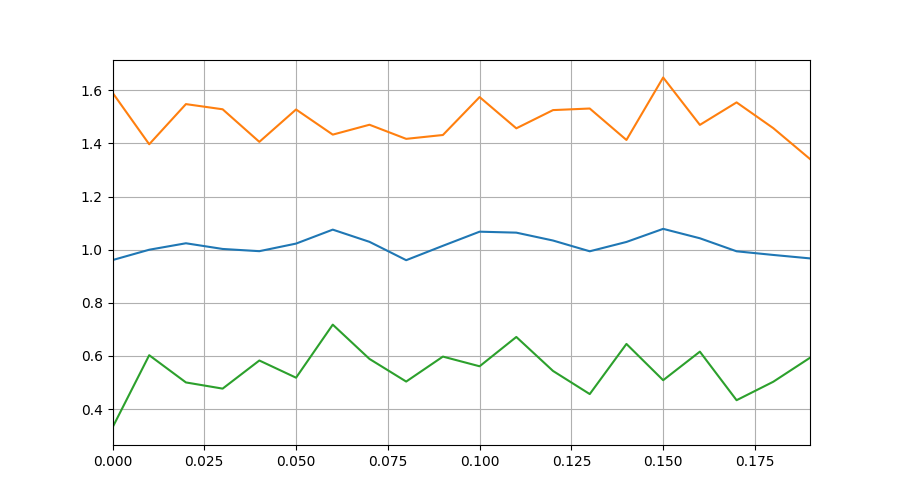
\includegraphics[width=\textwidth]{Assignment 1 - ML for TS (MVA 2023-2024)/bartlett_periodogram_N=200.png}}
    \centerline{Periodogram ($N=200$)}
    \end{minipage}
    \begin{minipage}[t]{0.3\textwidth}
    \centerline{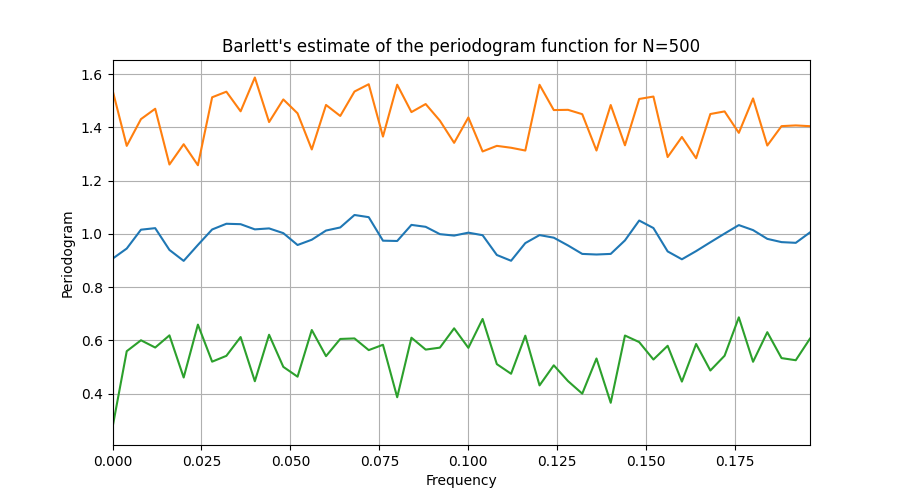
\includegraphics[width=\textwidth]{Assignment 1 - ML for TS (MVA 2023-2024)/bartlett_periodogram_N=500.png}}
    \centerline{Periodogram ($N=500$)}
    \end{minipage}
    \begin{minipage}[t]{0.3\textwidth}
    \centerline{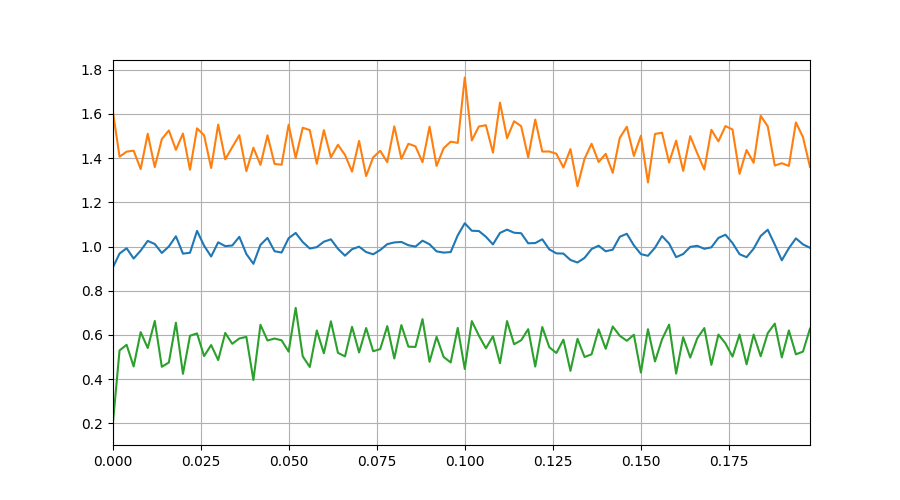
\includegraphics[width=\textwidth]{Assignment 1 - ML for TS (MVA 2023-2024)/bartlett_periodogram_N=1000.png}}
    \centerline{Periodogram ($N=1000$)}
    \end{minipage}
    \vskip1em
    \caption{Barlett's periodograms of a Gaussian white noise (see Question~\ref{q:barlett}).}
    \label{fig:barlett}
\end{figure}

\end{solution}
\section{Data study}

\subsection{General information}

\paragraph{Context.}
The study of human gait is a central problem in medical research with far-reaching consequences in the public health domain. This complex mechanism can be altered by a wide range of pathologies (such as Parkinson's disease, arthritis, stroke,\ldots), often resulting in a significant loss of autonomy and an increased risk of fall. Understanding the influence of such medical disorders on a subject's gait would greatly facilitate early detection and prevention of those possibly harmful situations. To address these issues, clinical and bio-mechanical researchers have worked to objectively quantify gait characteristics.

Among the gait features that have proved their relevance in a medical context, several are linked to the notion of step (step duration, variation in step length, etc.), which can be seen as the core atom of the locomotion process. Many algorithms have therefore been developed to automatically (or semi-automatically) detect gait events (such as heel-strikes, heel-off, etc.) from accelerometer and gyrometer signals.

\paragraph{Data.}
Data are described in the associated notebook.

\subsection{Step classification with the dynamic time warping (DTW) distance}

\paragraph{Task.} The objective is to classify footsteps then walk signals between healthy and non-healthy.

\paragraph{Performance metric.} The performance of this binary classification task is measured by the F-score.


\begin{exercise}
Combine the DTW and a k-neighbors classifier to classify each step. Find the optimal number of neighbors with 5-fold cross-validation and report the optimal number of neighbors and the associated F-score. Comment briefly.
\end{exercise}

\begin{solution}
The reported optimal $k$ is $7$, however, this estimate is not consistent as the F-scores for the different $k$'s are very close while being sensitive to the random process of splitting the dataset into two parts. The associated F-score is $0.87$.
\end{solution}

\newpage
\begin{exercise}\label{q:class-errors}
Display on Figure~\ref{fig:class-errors} a badly classified step from each class (healthy/non-healthy).
\end{exercise}

\begin{solution}
\begin{figure}
    \centering
    \begin{minipage}[t]{\textwidth}
    \centerline{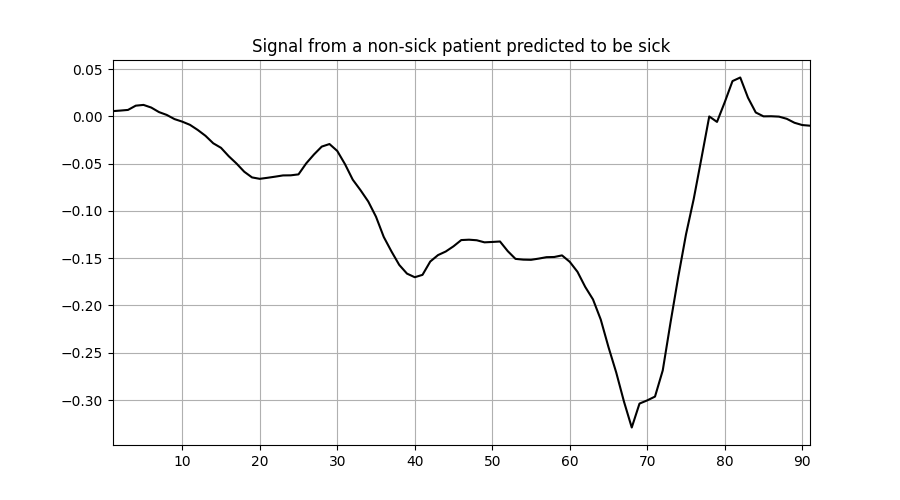
\includegraphics[width=0.6\textwidth]{Assignment 1 - ML for TS (MVA 2023-2024)/false_positive.png}}
    \centerline{Badly classified healthy step}
    \end{minipage}
    \vskip1em
    \begin{minipage}[t]{\textwidth}
    \centerline{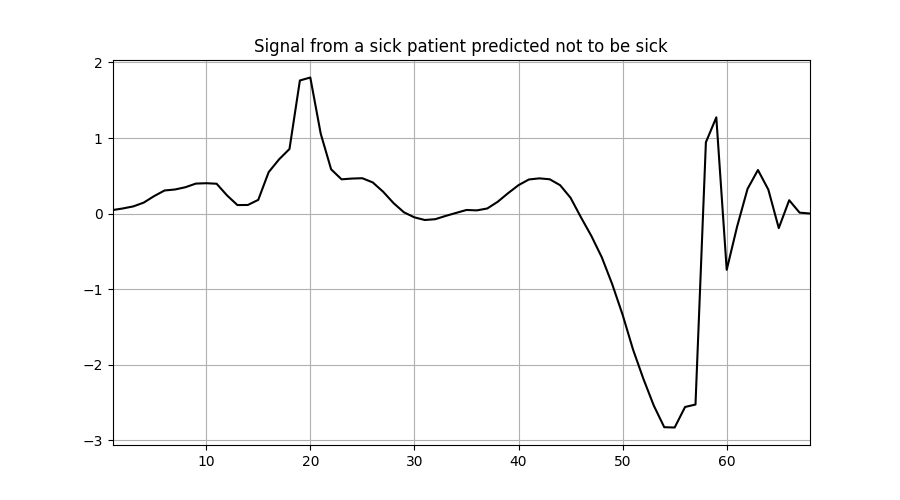
\includegraphics[width=0.6\textwidth]{Assignment 1 - ML for TS (MVA 2023-2024)/false_negative.png}}
    \centerline{Badly classified non-healthy step}
    \end{minipage}
    \vskip1em
    \caption{Examples of badly classified steps (see Question~\ref{q:class-errors}).}
    \label{fig:class-errors}
\end{figure}
\end{solution}


\end{document}
